\documentclass{article}
\usepackage{amsmath}
\usepackage{amssymb}
\usepackage{graphicx}
\usepackage{hyperref}
\usepackage[version=4]{mhchem}


\begin{document}
In \(\triangle A B C\), we have \(A C=B C=61\) and \(A B=22\). Suppose that \(D\) is a point on line \(A B\) such that \(B\) lies between \(A\) and \(D\) and \(C D=100\). What is \(B D\) ?\\
(A) 22\\
(B) 42\\
(C) 52\\
(D) 69\\
(E) 64\\
\centering
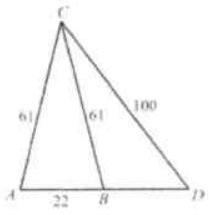
\includegraphics[width=\textwidth]{images/080.jpg}


Solution: (D).\\
Let \(C H\) be an altitude of \(\triangle A B C\). Applying the Pythagorean Theorem to \(\triangle C H B\) and to \(\triangle C H D\) produces\\
\(100^{2}-(x+11)^{2}=C H^{2}=61^{2}-11^{2}=60^{2}\), so \((x+11)^{2}=100^{2}-\) \(60^{2}=6400 \quad \Rightarrow \quad x+11=80\)\\
Thus \(B D=x=80-11=69\).\\
Note that 11-60-61 and 60-80-100 are all Pythagorean Triples.\\
\centering
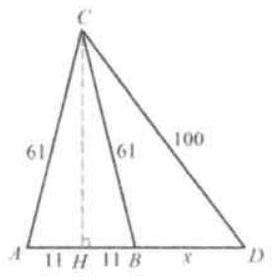
\includegraphics[width=\textwidth]{images/081.jpg}


\end{document}
